\chapter{ALICA Client}
\label{chap:ALICAClient}

The ALICA Client is a simple GUI for visualising AlicaEngineInfo messages. Currently it can be started for visualising the messages of a single engine by calling \verb#rosrun alica_client alica_client#. If you have several robots running, the GUI will flicker between their incoming messages. For visualising the messages of multiple robots you should use the Robot Control GUI (see~\ref{chap:RobotControl}). It integrates the same GUI component multiple times.

\begin{figure}[htbp]
 \centering
 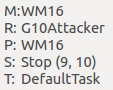
\includegraphics[scale=0.8]{img/AlicaClient.png}
 \caption{The ALICA Client GUI}
 \label{fig:ALICAClient}
\end{figure}

In Figure~\ref{fig:ALICAClient} you can see the ALICA Client GUI. \textbf{M:} denotes the currently executed master plan (WM16). \textbf{R:} denotes the current role of the robot (G10Attacker). \textbf{P:} is the deepest plan in the alica plan hierarchy, the robot is currently executing. As it is WM16, it means, that it is inside the master plan, but not deeper. Inside this plan, the robot is currently one of two robots inside the Stop state (\textbf{S:}). In this case, it is either the robot with id 9 or 10. The name of the task associated with the active state is the DefaultTask (\textbf{T:}).

This tool is definitely usefull for debugging ALICA plans, but please note, that the AlicaEngineInfo messages are only send roughly every 100ms, but the plan state of an ALICA Engine typically changes much faster, than that. Therefore, you want recognize agents racing through the plans' state machines. Making this visible needs a litte bit more sophisticated GUI, which should be able to read logs of the ALICA engine itself. Please see the \href{http://www.uni-kassel.de/eecs/fileadmin/datas/fb16/Fachgebiete/VS/Documents/ProjectsAndTheses/alica_client.pdf}{project description} for some details, about this possible bachelor project.



